% 2016 | UIBK
% vim:set spell tw=79:

\documentclass[article]{uibk}
\title{Analysing Parallel Programs using Constraint-Based-Analysis}
\author{Alex Hirsch}
\date{2017--01--09}

\addbibresource{references.bib}

\usepackage{caption}
\usepackage{wrapfig}

\usetikzlibrary{arrows.meta}
\usetikzlibrary{positioning}

\newenvironment{codebox}{\captionsetup{type=listing}}{}

\begin{document}

\maketitle

\section*{Abstract}
\label{sec:abstract}

Conventional data-flow analysis (DFA) is an established building block for
compile-time analysis, but it lacks context-sensitive information in its
vanilla form. Constraint-based analysis (CBA) is a more sophisticated approach,
providing such information, even when it comes to inter-procedural analysis
runs. This seminar-paper provides an introduction to the topic of data-flow
analysis including some background known. A uniform framework for the analysis
of programs with explicit, unbound, fork / join parallelism will be presented
in the main part, right after CBA has been explained.

\tableofcontents

\newpage

\section{Introduction}

This writeup will give a shallow introduction to data-flow analysis. While the
main focus lies on a mathematical model for analysing parallel programs, we
first start off with some required background knowledge, the control-flow graph
(CFG). The CFG is a crucial part when it comes to program analysis. Like many
other techniques found in compiler theory, program analysis commonly operates
on this graph. In addition to the explanation an example is provided within
this section.

Data-flow analysis, as the name already gives it away, is about analysing
\textit{properties} of an input program in a control-flow sensitive manner. But
some properties can be derived from the program using a simpler approach, the
flow-insensitive analysis. While it is not really necessary to know about
flow-insensitive analysis in order to talking about data-flow analysis it may
ease the introduction to the topic for the unfamiliar reader. The two extrema,
Andersen-style Analysis and Steensgaard Analysis, will be explained together
with a tiny example.

A short primer on data-flow analysis will be given next, utilizing what has
already been mentioned up to this point. An important concept for these kind of
analyses is the mathematical structure of a lattice, which will accompany us on
our journey. A few paragraphs will explain the concept followed by some common
examples for data-flow analysis. After this the reader should be familiar with
the basic concept and how things are supposed to fit together. Although there
may still be some details left untouched. If this bothers you I suggest taking
a peak at the provided references, especially \cite{Nielson:ppa}.

After a glimpse at bit vector problems, a more sophisticated approach, the
constraint-based approach is presented. Followed by illustrating a way to use
it on input programs with parallel constructs. Last but not least the concept
of \textit{effect analysis} is touch followed by a short conclusion.

\subsection{Motivation}

Program analysis in general is a big topic not only in compiler theory.
Extracting certain properties directly, automatically from an input program can
be viable for multiple of use-cases. When talking about compilers, most of
their optimization frameworks rely on some kind of data-flow analysis to
identify structures in their input, which can be transformed safely to yield
more efficiency (with respect to power consumption, memory usage, runtime
or a combination of them).

Since our programming focuses more and more on parallel and distributed
systems, also our compilers need to be aware of these concepts in order to run
relevant checks, produce correct output code and perform optimizations in
similar fashion to sequential programs.

The main challenge here arises from complexity of analysis parallel programs.
Even having only a very small part of the program run in parallel can yield an
enormous increase in complexity for the analysis. The number of possible
execution paths a program can experience at runtime grows exponentially with
the number of parallel directives (i.e.\ fork).

While most data-flow analysis already only compute approximations which such an
increase in search-space a useful result will be even harder to achieve.

\subsection{Related Work}

The general topic of data-flow analysis, including required background
knowledge, is commonly encountered in University compiler lectures. Therefore
slide decks available online together with Wikipedia pose an acceptable, easy
to understand source of information. A more in-depth experience can be gained
by looking at \cite{herbert_phd} and \cite{Nielson:ppa}.

While there are multiple papers targeting the topic of analysing parallel
programs using the aforementioned technique, the one that sticks out is
\cite{parallel_cba}. Its mathematical approach goes hand in hand with
\cite{Nielson:ppa} and provides a well defined basis.

\subsection{Control-flow Graph}

The control-flow of a program can be represented as a graph, in which each node
typically represents a \textit{basic block}. A basic block is a sequence of
instructions without any jumps or jump targets (labels) in-between --- it
commonly begins with a jump target and ends with a jump instruction. Jumps from
one basic block to another are translated to directed edges in the control-flow
graph (CFG). An edge that directs to an already met block (during depth-first
traversal) is referred to as \textit{backward edge} and most of the time
introduced by a loop. Adding two additional blocks, the \textit{entry block}
and \textit{exit block} can help keeping the implantation of algorithms
(operating on the graph) simple. All control-flows start at the entry block and
end at the exit block.~\cite{wiki:cfg}

\begin{wrapfigure}[15]{r}{0.37\textwidth}
    \vspace{-1.4em}
    \centering
    %\usetikzlibrary{arrows.meta}
%\usetikzlibrary{positioning}

\tikzstyle{ptr} = [-{Latex[length=2.7mm]}]

\tikzstyle{loop} = [ptr,looseness=10]

\tikzstyle{block} = [
    draw,
    align=center,
    rectangle,
    minimum height=0.8cm,
    minimum width=1.6cm
]

\begin{tikzpicture}

    % main
    \node[block] (1) {\ttfamily main:};
    \node[block] (2) at (-1.5,-1.4) {\ttfamily print\_usage()};
    \node[block] (3) at ( 1.5,-1.4) {\ttfamily print\_something(\dots)};
    \node[block] (4) [below = 2cm of 1] {\ttfamily return};
    \path[ptr] (1) edge (2)
               (1) edge (3)
               (2) edge (4)
               (3) edge (4);

    % print_usage
    \node[block] (5) [below = of 4] {\ttfamily print\_usage:};
    \node[block] (6) [below = of 5] {\ttfamily puts(\dots)};
    \node[block] (7) [below = of 6] {\ttfamily return};
    \path[ptr] (5) edge (6)
               (6) edge (7);

    % print something
    \node[block] (8)  [below = of 7] {\ttfamily print\_something:};
    \node[block] (9)  [below = of 8] {\ttfamily puts(\dots)};
    \node[block] (10) [below = of 9] {\ttfamily return};
    \path[ptr] (8) edge (9)
               (8) edge[bend left = 60pt] (10)
               (9) edge[loop left] (9)
               (9) edge (10);

\end{tikzpicture}

    \caption{Control-Flow Graph of \texttt{cfg.c}}
    \label{fig:cfg}
\end{wrapfigure}

What exactly composes a node of a CFG is not set in stone and varies depending
on the actual application. While the textbook definition concerns itself with
basic blocks, one could easily abstract away whole functions in a graph's
nodes. This is somewhat true even for its edges. Based on the application edges
can carry additional information. We will encounter such an extended
control-flow graph later on.

\Cref{src:cfg} displays a short C program with 3 functions. \Cref{fig:cfg}
illustrates the corresponding CFG. Each of the functions features a dedicated
entry (function name) and exit (\texttt{return}) block. The example contains
branching as well as loops. Note that from this CFG the original program cannot
be reconstructed fully since some details have been omitted (i.e.\ loop-index
and condition checking in \texttt{print\_something}).

\begin{codebox}
    \cfile{src/cfg.c}
    \vspace{-1.5em}
    \caption{Control-Flow Graph Example \texttt{cfg.c}}
    \label{src:cfg}
\end{codebox}

During a program analysis run certain properties are tracked across the CFG's
nodes. These properties (e.g.\ reaching definition) are recorded when a node is
entered or left. These records are annotated by the labels of the related graph
node together with either $in$ or $out$. For instance, $REACH_{in}[S]$ is the
reaching definition record at the entry point of the graph node labelled
$S$.~\cite{wiki:reaching_definition}

This syntax is often shortened to $in(S)$ / $out(S)$ when the analysis kind can
be derived from the current context. But more about this in
\Cref{sec:dataflow}.

\subsection{Flow-insensitive Analysis}

Before talking about conventional data-flow analysis, a more naive approach to
program analysis is presented. A flow-sensitive analysis takes the order of
statements into account, while a flow-insensitive analysis does not. Hence for
flow-insensitive analysis information does not need to be computed (and
re-evaluated) at every point of the program. It is therefore cheaper to perform
but also less precise. The solution produced by a flow-insensitive analysis is
valid for the whole program. Pointer analysis are common examples and two of
them are mentioned next.

Note that this topic can be found in most of the relevant text books, what is
presented here is mainly taken from \cite{slides:flow-insensitive} and
\cite{wiki:pointer-analysis}.

The goal of a pointer analysis is to find which pointer (or reference) can
point to which variable (or storage location). The two algorithms we will look
at are the Andersen-style analysis and Steensgaard analysis. Andersen-style
features a more precise solution, yet is more expensive to compute, while
Steensgaard's way is near-linear but imprecise. These are the two extrema, all
other flow-insensitive pointer analyses are hybrids of them.

\paragraph{Andersen-style Analysis}

Pointer (or reference) assignments will be modeled as constraints, which are
utilized to propagate information about pointer targets. Three different types
of constraint of varying complexity are used to generate a constraint graph.
Each node in this constraint graph corresponds to one variable, each edge to
one constraint. Indirect constraints are resolved, yielding new edges until a
fixed point is reached. The solution is attained by computing the transitive
closure of the graph.

\paragraph{Steensgaard Analysis}

In Andersen-style Analysis information flows from the right-hand side of a
constraint to the left-hand side --- Steensgaard uses equality constraints
instead, which is less precise but allows information to flow both ways which
allows for a much faster computation. At its core the \textit{Union-Find} data
structure is used. Inverted trees\footnote{A tree where each node has a pointer
to its parent} are used to hold the current state of the computation, where the
root element is used as a representative for the whole tree. Processing a
constraint of the form $x = y$ will result in a merge of the tree containing
$x$ and the tree containing $y$.

\paragraph{Pointer Analysis Example}

Following code segment has been analyzed with the mentioned algorithms. The
results are shown in \Cref{fig:pointer_analysis} --- Andersen-Style gives us
the more detailed solution where $b$ only points to $c$ and $d$ only points to
$e$, while Steensgaard tells us $a$ points to $b$ and $d$, which then point to
$c$ and $e$.

\newpage

\begin{wrapfigure}[7]{r}{0.55\textwidth}
    \centering
    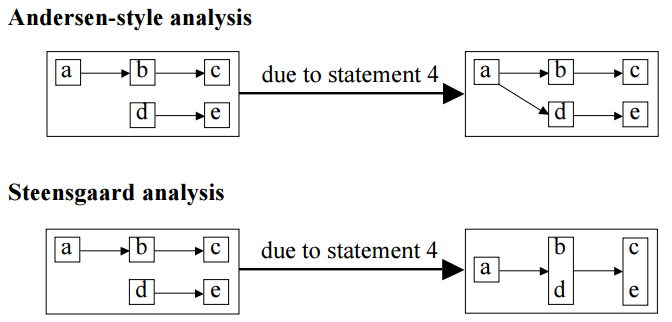
\includegraphics[width=0.55\textwidth]{gfx/pointer_analysis.png}
    \caption{Andersen-Style vs. Steensgaard Example}
    \label{fig:pointer_analysis}
\end{wrapfigure}

The difference between the to algorithms is further illustrated in
\cref{fig:pointer_analysis}. There one can see both analyses with identical
input (the program given below) followed by two similar, yet different in
detail solutions for the pointer aliasing.

\begin{ccode}
    int **a, *b, c, *d, e;
    1: a = &b;
    2: b = &c;
    3: d = &e;
    4: a = &d;
\end{ccode}

\section{Data-flow Analysis}
\label{sec:dataflow}

In this section, the basis of data-flow analysis will be described. Generally
speaking their are two common approaches. The first, more common one, is the
\textit{equational} approach in which a system of equations is constructed and
solved to model and reason about program properties. The second approach
utilizes \textit{constraints} between points of a program and is therefore
known as the \textit{constraint-based} approach.

As the reader may have guessed already by the name, the (control-)flow of the
program is quite important for these kind of analyses --- and while one could
work on the abstract syntax tree (AST), using a CFG is often much simpler and
yields similar outcome (with respect to data-flow analysis). At its core lies a
framework for proving facts about programs. \textit{Facts} are extracted from
the CFG by traversing it and looking at all paths through the
program.~\cite{slides:dataflow}

Depending on the analysis, traversal can be either \textit{forward} or
\textit{backward}. Each block in the CFG is associated with two \textit{program
points}, one just before the block $S$ is executed ($in(S)$), the other right
after the block has been executed ($out(S)$). In a forward data-flow analysis,
data \emph{flows} from $in$ to $out$, for backward data-flow analysis the other
way round. Most data-flow analyses can be realized using only one direction of
traversing the CFG, but there exist also few which require bidirectional flow.

More interesting are the points where two branches of the CFG meet (either in
forward or backward traversal). Again there are two ways an analysis can work.
It can be either a \textit{must} analysis or a \textit{may} analysis. A
\textit{must} analysis requires that a property must hold in all branches to be
still considered after the meeting point (logical-and). Alternatively, in a
\textit{may} analysis, the property is considered after the meeting point if
it holds in at least one branch (logical-or).

Most facts extracted by such an analysis form a \textit{lattice}. Because of
this we will now take a short detour and look at the mathematical concept of a
lattice.

\subsection{Lattice}

% TODO partially ordered set footnote

\begin{wrapfigure}[9]{r}{0.3\textwidth}
    \vspace{-6em}
    \centering
    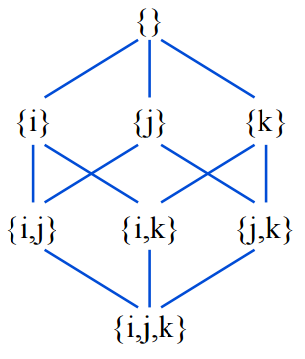
\includegraphics[height=16em]{gfx/lattice.png}
    \caption{Lattice Example}
    \label{fig:lattice}
\end{wrapfigure}

A \textit{lattice} is an algebraic structure which consists of a partially
ordered set in which every two elements have a unique least upper bound
(\textit{join}) and a unique greatest lower bound (\textit{meet}). Its purpose
with respect to program analysis is to model a domain of program properties.
The \textit{height} of a lattice is given by the longest path though partial
order from greatest to least. Elements of the lattice will represent flow
values ($in$ and $out$ sets) while $\top$ and $\bot$ represent the
\textit{best-case} and \textit{worst-case} information respectively. The
\textit{meet} operator $\sqcap$ describes how two flow values are
merged.~\cite{wiki:lattice,slides:lattice,slides:lattice2}

\Cref{fig:lattice} shows an example application for a lattice where three
variables $i$, $j$ and $k$ are given and a flow value can exhibit any
combination of them. Hence the $\top$ and $\bot$ value can be mapped to all
variables and $\emptyset$ respectively. The height of the lattice, $4$, is
immediately deduced from the illustration and the ordering of the lattice
($\sqsubseteq$) is mapped to $\subseteq$.

There exists also the concept of a \textit{semilattice}, which resembles a
normal lattice, but only features \emph{either} a least upper bound \emph{or}
greatest lower bound. Each variant is referred to with their own name
\textit{join-semilattice} or \textit{meet-semilattice}.

See \cite{lattice_tutorial} for a more comprehensive introduction to lattices.

\subsection{Common Data-flow Analysis}

Before we continue with a more detailed example and the constraint-based
approach, two simple data-flow analyses are presented commonly found in
textbooks.

\paragraph{Reaching Definitions}

A definition at program point $p_1$ \textit{reaches} program point $p_2$ if there
is a control-flow path from $p_1$ to $p_2$ along which the variable defined by
$p_1$ is not redefined.~\cite{wiki:reaching_definition}

\begin{minipage}[t]{0.45\textwidth}
    \begin{code*}{linenos=false}
        p1: x = 42
        p2: y = 12
        p3
    \end{code*}

    The definition from $p_1$ reaches the program point $p_3$.
\end{minipage}\hfill
\begin{minipage}[t]{0.45\textwidth}
    \begin{code*}{linenos=false}
        p4: z = 24
        p5: z = 16
        p6
    \end{code*}

    The definition of $p_4$ does not reach $p_6$. It is \textit{killed} by the
    definition at $p_5$.
\end{minipage}
\vspace{2em}

In terms of data-flow equations, this can be written as
%
\begin{align*}
    in(b)  &= \bigcup_{p \in pred(b)} out(p) \\
    out(b) &= gen(b) \cup (in(b) - kill(b))
\end{align*}
%
where $gen(b)$ is the set definitions generated in $b$ and $kill(b)$ the set of
definitions \textit{killed} in $b$. Also this is a forward may analysis.

\paragraph{Liveness Analysis}

A variable $v$ is live at program point $p$ iff there exists a path from $p$ to
some \emph{use} of $v$ along which $v$ is not redefined.~\cite{wiki:liveness}

\begin{minipage}[t]{0.45\textwidth}
    \begin{code*}{linenos=false}
        p1: a = 2
        p2: b = 3
        p3: x = a * b
    \end{code*}

    Variables $a$ and $b$ are \textit{live} at program point $p_3$.
\end{minipage}\hfill
\begin{minipage}[t]{0.45\textwidth}
    \begin{code*}{linenos=false}
        p4: c = 2
        p5: d = 7
        p6: y = c * c
    \end{code*}

    Only variable $c$ is \textit{live} at program point $p_6$ since $d$ is not
    \textit{used} in $p_6$ or later on.
\end{minipage}
\vspace{2em}

These would be the related data-flow equations.
%
\begin{align*}
    out(b) &= \bigcup_{s \in succ(b)} in(s) \\
    in(b)  &= gen(b) \cup (out(b) - kill(b))
\end{align*}
%
Here $gen(b)$ and $kill(b)$ represent which variables are used before an
assignment and which variables are assigned to, respectively. Contrary to
reaching definition, this is a backward may analysis.

%\subsubsection{Constant Propagation}
%
%Together with constant folding, expressions can be simplified along the control
%flow.
%
%\begin{minipage}[t]{0.45\textwidth}
%    \begin{code*}{linenos=false}
%        p1: a = 12
%        p2: b = a + 24;
%    \end{code*}
%
%    Original code.
%\end{minipage}\hfill
%\begin{minipage}[t]{0.45\textwidth}
%    \begin{code*}{linenos=false}
%        p1: a = 12
%        p2: b = 32;
%    \end{code*}
%    Constant folding and propagation has been applied.
%\end{minipage}

\subsection{Bit Vector Problems}

Some problems, like reaching definition, can be efficiently modelled as
\textit{bit vectors}. One vector is associated with each program point, and
(for reaching definition) each bit corresponds to a definition. The value of
the bit indicates whether the definition reaches the current program point. The
analysis can leverage bitwise operations to efficiently operate on these
vectors. A typical join operation would be set union and can be implemented by
a bitwise \textit{logical or}.~\cite{wiki:dfa}

In case of the live-variable analysis:

\vspace{-1.5em}
\begin{minipage}[t]{0.45\textwidth}
    \begin{align*}
        out(b) &= \bigcup_{s \in succ(b)} in(s) \\
        in(b)  &= gen(b) \cup (out(b) - kill(b))
    \end{align*}
\end{minipage}\hfill
\begin{minipage}[t]{0.45\textwidth}
    \vspace{1.5em}
    \begin{code*}{linenos=false}
        for s in succ(b):
            out(b) = out(b) | in(s)
        in(b) = (out(b) & ~kill(b)) | gen(b)
    \end{code*}
\end{minipage}

\subsection{Example}

\begin{wrapfigure}[5]{r}{0.4\textwidth}
    \vspace{-1.4em}
    \centering
    %\usetikzlibrary{arrows.meta}
%\usetikzlibrary{positioning}

\tikzstyle{ptr} = [-{Latex[length=2.7mm]}]

\tikzstyle{loop} = [ptr,looseness=10]

\tikzstyle{block} = [
    draw,
    align=center,
    rectangle,
    minimum height=0.8cm,
    minimum width=1.6cm
]

\begin{tikzpicture}

    \node[block] (1) {\ttfamily y = x};
    \node[block] (2) [below = of 1] {\ttfamily z = 1};
    \node[block] (3) [below = of 2] {\ttfamily y > 1};
    \node[block] (4) at (-2,-5.5) {\ttfamily z = z * y};
    \node[block] (5) [below = of 4] {\ttfamily y = y - 1};
    \node[block] (6) at (2,-5.5) {\ttfamily y = 0};

    \path[ptr] (1) edge (2)
               (2) edge (3)
               (3) edge node[midway,left]  {true}  (4)
               (3) edge node[midway,right] {false} (6)
               (4) edge (5);

    \draw[ptr] (5.south) |- ++(-1.5,-0.5) |- (3.west);

    \foreach \x in {1,...,6}
        \node at ($(\x.east)+(0.25,0)$) {\x};

\end{tikzpicture}

    \caption{Control-Flow Graph of \mbox{\texttt{factorial.c}}}
    \label{fig:factorial}
\end{wrapfigure}

Let's take the following program computing $x!$ together with the corresponding
CFG in \cref{fig:factorial}. Note that we will only focus on the calculating
part here and assign each statement its own block for
simplicity.~\cite{Nielson:ppa}

\begin{codebox}
    \cfile{src/factorial.c}
    \vspace{-1.5em}
    \caption{Control-Flow Graph Example \texttt{cfg.c}}
    \label{src:cfg}
\end{codebox}

\vspace{1.5em}

Running a Reaching Definition analysis on this code results in the following
twelve equations, two for each block.
%
\begin{align*}
    in(1) &= \{(x,?)\}          & out(1) &= \{(y,1)\} \cup (in(1) - \{(y,l) \mid l \in Label\}) \\
    in(2) &= out(1)             & out(2) &= \{(z,2)\} \cup (in(2) - \{(z,l) \mid l \in Label\}) \\
    in(3) &= out(2) \cup out(5) & out(3) &= in(3) \\
    in(4) &= out(3)             & out(4) &= \{(z,4)\} \cup (in(4) - \{(z,l) \mid l \in Label\}) \\
    in(5) &= out(4)             & out(5) &= \{(y,5)\} \cup (in(5) - \{(y,l) \mid l \in Label\}) \\
    in(6) &= out(5)             & out(6) &= \{(y,6)\} \cup (in(6) - \{(y,l) \mid l \in Label\})
\end{align*}
%
Each pair consists of a variable ($x$, $y$, $z$) and a label, where the label
is either the number of the block or `$?$' if the variable is not initialized
within this context, hence it can be considered an input to the program. When
focusing at block $3$, one can see that since no variable is modified,
the information flowing into the block is the same as flowing out of the block.
Even further at block $3$ two different control flows meet yielding a merge of
facts.

While there are multiple solutions satisfying this system of equations, we are
only interested in one of them. Fortunately these solutions are ordered and the
\textit{least} solution contains the fewest pairs of reaching definitions that
is consistent with the program. This will not only give us a correct solution,
but also the most precise one.

\subsection{Constraint-based Analysis (CBA)}

Previously we dealt with extracting multiple equations from a CFG by traversing
it, and then solving a system of equations to derive information (program
properties / facts) about the program. Behind the scenes the extracted
equations are linked together by constraints which have been processed
implicitly. The main idea behind the constraint-based approach is to directly
extract these constraint and handle them explicitly, instead of the original
data-flow equations.~\cite{Nielson:ppa,herbert_phd}

Reusing the example from above (\cref{fig:factorial}) the following list of
constraints can be derived.
%
\begin{align*}
    out(1) &\supseteq in(1) - \{(y,l) \mid l \in Label\} &
    out(1) &\supseteq \{(y,1)\} \\
    out(2) &\supseteq in(2) - \{(z,l) \mid l \in Label\} &
    out(2) &\supseteq \{(z,2)\} \\
    out(3) &\supseteq in(3) \\
    out(4) &\supseteq in(4) - \{(z,l) \mid l \in Label\} &
    out(4) &\supseteq \{(z,4)\} \\
    out(5) &\supseteq in(5) - \{(y,l) \mid l \in Label\} &
    out(5) &\supseteq \{(y,5)\} \\
    out(6) &\supseteq in(6) - \{(y,l) \mid l \in Label\} &
    out(6) &\supseteq \{(y,6)\}
\end{align*}
%
Investigating this list and the original program closely a pattern emerges. For
this example every time a variable is assigned, two constraints are generated,
one for excluding all pairs $(x,\_)$ from a block's entry set and one for
adding a new pair related to this assignment $(x,l)$. Otherwise, if no variable
is assigned, everything is simply passed through.

Now these constraints only tell us how information flows \emph{through} each
block, we are still missing how information flows \emph{between} blocks.
Therefore the following list is derived.
%
\begin{align*}
    in(2) &\supseteq out(1) \\
    in(3) &\supseteq out(2) & in(3) &\supseteq out(5) \\
    in(5) &\supseteq out(4) \\
    in(6) &\supseteq out(3)
\end{align*}
%
Again a pattern is immediately visible, each edge in the CFG results in a
constraint connecting the exit set of block with the entry set of its
successor.

The last constraint we need is introducing our input to the program.
\[
    in(1) \supseteq \{(x,?)\}
\]

The least solution to this system of constraints is the same solution as the
one to the original system of equations presented previously.

% TODO
%\subsection{Benefits of CBA}
%
%Since the constraints are explicit in CBA their generation and their solving
%can be separated, yielding a more flexible generation process. Even further
%constraints can be generated on-the-fly and solved as needed.

\newpage

\section{CBA on Parallel Programs}

Up until now we have only dealt with sequential programs. In this section one
approach to analysing parallel programs will be presented. The section is
started by a naive approach to detecting race conditions and extending the CFG
with some parallel directives. The main focus lies on a technique for modelling
\textit{interleaved} control-flow and extracting the effects of certain
procedures.

But first let us consider a basic example in which we straightforwardly
identify a race condition in the similar manner reaching definitions were
analysed.

\vspace{-1em}
\begin{minipage}[t]{0.45\textwidth}
    \begin{figure}[H]
        \centering
        %\usetikzlibrary{arrows.meta}
%\usetikzlibrary{positioning}

\tikzstyle{ptr} = [-{Latex[length=2.7mm]}]

\tikzstyle{loop} = [ptr,looseness=10]

\tikzstyle{block} = [
    draw,
    align=center,
    rectangle,
    minimum height=0.8cm,
    minimum width=1.6cm
]

\begin{tikzpicture}

    \node[block] (1) {\ttfamily x = 1};
    \node[block] (2) at (-1,-1.5) {\ttfamily x = 2};
    \node[block] (3) at ( 1,-1.5) {\ttfamily x = 3};
    \node[block] (4) [below = 2.2cm of 1] {\ttfamily return x};

    \path[ptr,dashed] (1) edge (2)
                      (1) edge (3)
                      (2) edge (4)
                      (3) edge (4);

    \foreach \x in {1,2,4}
        \node at ($(\x.west)-(0.25,0)$) {\x};
    \node at ($(3.east)+(0.25,0)$) {3};

\end{tikzpicture}

        \caption{Race Condition Example}
        \label{fig:race_condition}
    \end{figure}
\end{minipage}
\begin{minipage}[t]{0.45\textwidth}
    \vspace{2em}
    \begin{align*}
        \mathcal{V}_1(x) &= \{1\} \\
        \mathcal{V}_2(x) &= \{2\} \\
        \mathcal{V}_3(x) &= \{3\} \\
        \mathcal{V}_4(x) &= \mathcal{V}_2(x) \cup \mathcal{V}_3(x) = \{2,3\}
    \end{align*}
\end{minipage}
\vspace{1em}

In \cref{fig:race_condition} we see a CFG, in which blocks 2 and 3 can be
executed in parallel. In this example this is indicated by the dashed edges.
Now utilizing data-flow analysis in a similar manner to the already provided
examples we can easily identify the value of $x$ in each block. As state by the
equations right beside the CFG --- $\mathcal{V}_b(x)$ gives a set of values
$x$ can have at block $b$. We can observe that in the last case, block 4, the
assignments of the two predecessors are merged, yielding a set of size $2$ as
result. In other words, when executing this program, block 2 could be executed
either \emph{before} or \emph{after} block 3. Both cases yield a different
outcome, hence the static analysis can only determine the result will be either
$2$ or $3$. Therefore we have successfully found a race condition.

\subsection{Parallel Execution Paths}

The first example provided in this section was kept very in-formal to ease the
introduction. Next we will examine the underlying constraints more carefully.
Take the CFG provided by \cref{fig:parallel_paths}. The program described
consists of 3 functions, $main$, $p$ and $q$. Annotated edges indicate that
either a single function is called ($p$) or that two functions are called in
parallel ($p \parallel q$). A non-annotated edge is referred to as a
\textit{basic} edge.~\cite{parallel_cba}

% TODO tikzify
\begin{figure}[H]
    \centering
    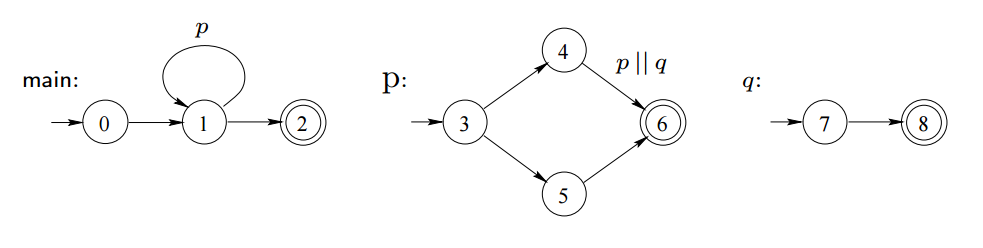
\includegraphics[width=0.8\textwidth]{gfx/parallel_paths.png}
    \caption{CFG for Parallel Paths Example}
    \label{fig:parallel_paths}
\end{figure}

The next step is to model the different, possible execution paths happening at
runtime (because of the scheduling of parallel executions). This is formalized
by an \textit{interleaving semantics}, which is defined by a series of
mathematical expressions in the original paper.~\cite{parallel_cba}

Basically you start off with two sets and a sequence of edges (word). Each edge
can be mapped to either one of the two sets. Doing this for all possible
combinations gives you all possible \textit{interleavings} of the sequence when
you combine the two sets. In addition to this a function $pre$ is defined which
returns all prefixes of words in one set.

The following possible executions paths are considered in the original paper:

% TODO same level execution path

\begin{itemize}
    \item For a procedure $p$, the set $\Pi(p)$ of all execution paths for $p$;
    \item For a program point $v$ in procedure $p$, the set $\Pi(v)$ of all
        paths starting at the entry point of $p$ and reaching $v$ (on the same
        level)
    \item For every procedure $p$, the set $\Pi_r(p)$ of all paths starting at
        a call of \textit{main} and reaching some call of $p$.
    \item For every program point $v$, the set $\Pi_r(v)$ of all paths starting
        at a call of \texttt{main} and reaching program point $v$.
\end{itemize}

A constraint system is presented next, which least solution corresponds the
considered execution paths.

% TODO what is cdot

\begin{align}
    \Pi(p) &\supseteq \Pi(r)                                   && \text{$r$ return point of $p$} \\
    \Pi(s) &\supseteq \{\epsilon\}                             && \text{$s$ entry point of a procedure} \\
    \Pi(v) &\supseteq \Pi(u) \cdot \{e\}                       && \text{$e = (u,v)$ basic edge} \\
    \Pi(v) &\supseteq \Pi(u) \cdot \Pi(p)                      && \text{$e = (u,v)$ calls $p$} \\
    \Pi(v) &\supseteq \Pi(u) \cdot (\Pi(p_1) \otimes \Pi(p_2)) && \text{$e = (u,v)$ calls $p_1 \parallel p_2$}
\end{align}

The first 4 lines determine the sets of all \textit{same-level} execution
paths, as known from inter-procedural analysis of sequential programs.
Line (4) states that for every edge $e = (u,v)$ calling a procedure $p$, the
set of same-level execution paths reaching $u$ extended by any execution path
through the procedure $p$. Line (5) for parallel call of $p_1 \parallel p_2$
has the same form as line (4), but now the same-level execution paths to the
program point before the call are extended by all interleavings of execution
paths for $p_1$ and $p_2$.

Next auxiliary sets $\Pi(u,p)$ are introduced where $v$ is a program point and
$p$ a procedure. They give the sets of executions paths reaching $v$ from a
call of $p$, are necessary to specify the sets $\Pi_r(p)$ and $\Pi_r(v)$ which
will be needed later and defined as the least solution of the following
constraint system:

\begin{align}
    \Pi(v,q) &\supseteq \Pi(v)                               && \text{$v$ program point of procedure $q$} \\
    \Pi(v,q) &\supseteq \Pi(u) \cdot \Pi(v,p)                && \text{$e = (u,\_)$ calls $p$ in $q$} \\
    \Pi(v,q) &\supseteq \Pi(u) \cdot (\Pi(v, p_i) \otimes M) && \text{$e = (u,\_)$ calls $p_1 \parallel p_2$ in $q$}
\end{align}

where $M$ in line (3) is given by $M = pre(\Pi(p_3 - i))$. Line (6) tells us
that for a procedure $q$ with program point $v$ the set of execution paths from
$q$ to $v$ subsumes all same-level execution paths from $q$ to $v$. In the next
line (7) whenever an edge $e = (u,\_)$ in the body of a procedure $q$ is
calling another procedure $p$, the set of execution paths from $q$ to $v$
subsumes all computation paths consisting of a same-level execution path from
$q$ to the program point $u$ followed by an execution path from $p$ to $v$.
Lastly, line (8) considers a parallel call of $p_1$ and $p_2$ in the body of
$q$. Afterwards we have to append to the same-level execution paths to $u$ all
interleavings of execution paths from $p_i$ to $v$ with prefixes of same-level
execution paths for the parallel procedure.

Now given this auxiliary set the values $\Pi_r(v)$ and $\Pi_r(p)$ can be
defined by the least solution of:

\begin{align}
    \Pi_r(v) &\supseteq \Pi(v, \texttt{main}) && \text{$v$ a program point} \\
    \Pi_r(p) &\supseteq \Pi_r(u)              && \text{edge $(u,\_)$ calls $p$, $p \parallel \_$ or $\_ \parallel p$}
\end{align}

\subsection{Effect Analysis}

$\mathbb{D}$ is a complete lattice and represents the set of abstract
properties observed by an analysis. $\mathbb{F}$ describes all possible ways
how properties may be transformed when passing from one program point to
another. It is a subset of monotonic functions from $\mathbb{D}$ to
$\mathbb{D}$ and contains the constant $\bot$ function and the identity
function. Furthermore it is closed under composition. $\mathbb{D}$ as well as
$\mathbb{F}$ can be infinite. There are a few more restrictions but they are
omitted for clarity.~\cite{parallel_cba}

We can now draw parallels to the bit vector section provided earlier. Remember
that some common data-flow analysis can be modeled as bit vector problems to be
handle efficiently. In these cases, we can choose $\mathbb{D} = \mathbb{B}^h$
where $\mathbb{B} = \{0 \sqsubset 1\}$ and $h$ will be the height of the
lattice.

For other data-flow analysis, which cannot be modeled as bit vector problems,
like constant propagation we may choose, for instance, $\mathbb{D} = V \to
\mathbb{V}$ where $V$ is the set of program variables and $\mathbb{V}$ is the
flat lattice of possible values for program variables. An abstract value $d \in
\mathbb{D}$ therefore represents and assignment of variables to values.

Next we map functions to edges of our control-flow graph to model its effect on
our properties. Therefore let $E$ denote the set of edges and $[.] : E \to
\mathbb{F}$ denote an assignment of functions to edges. Furthermore $[.]$ will
be extended to sequences and sets.

\begin{align*}
    [w] = [e_n] \circ \dots \circ [e_1] && [M] = \bigsqcup\;\{[w] | w \in M\}
\end{align*}

Functions $[w]$ and $[M]$ are also called the \textit{effect} of the sequence
$w$ and the set $M$, respectively. Even further the program analysis tries to
compute (approximate) the effects of procedures. This is done by computing
$[\Pi(p)]$ for each procedure $p$, given an assignment for all basic edges.
Furthermore this computation is \textit{merged over all paths}. Note that the
set of possible execution paths is quite big, hence the solution may not be
computable efficiently.

To work around this, the conventional approach is to setup a set $C$ of
constraints on the values we are interested in and then choose constraints such
that the any solution to $C$ is guaranteed to be a safe approximation. The
solution found this way is often equal to the \textit{meet-over-all-paths}
solution (\textit{coincidence}).

The following constraint system is provided next to model the effect analysis
as a constraint-based analysis.

\begin{align}
    [p] &\sqsupseteq [r]                             && \text{$r$ return point of $p$} \\
    [s] &\sqsupseteq I                               && \text{$s$ entry point} \\
    [v] &\sqsupseteq f_e \circ [u]                   && \text{$e = (u,v)$ basic edge} \\
    [v] &\sqsupseteq [p] \circ [u]                   && \text{$e = (u,v)$ calls $p$} \\
    [v] &\sqsupseteq ([p_1] \otimes [p_2]) \circ [u] && \text{$e = (u,v)$ calls $p_1 \parallel p_2$}
\end{align}

Similar to before the first 4 lines determine the effects of procedures as
known from inter-procedural analysis of sequential programs. In line (11) the
effect of a procedure $p$ is equal to what has been accumulated for its return
point. The next line (12) indicates that accumulation of effects start at the
entry point of a procedure with the identity function $I$. Line (13) tells us
that the contribution of a basic edge $e = (u,v)$ to the value for $v$ is given
by the value for $u$ extended by the application of the function associated
with $e$. It follows in line (14) that the contribution of a calling edge $e =
(u,v)$ is similar to line (13) but the associated function $f_e$ is replaced
with the effect of the called procedure $[p]$. Finally line (5) for parallel
calls has the same form, but the effect of both procedures $p_1$ and $p_2$ have
to be combined using the interleaving operator $\otimes$.

Utilizing this framework we have shown a way to analyse programs featuring
parallel directives like fork / join in a generic fashion.

\section{Conclusion}

In the past few pages an introduction the basics of data-flow analysis was
given with a final focus on analysis parallel programs. The more sophisticated
constraint-based approach has been provided as an extension to conventional
data-flow analysis. Even further we touched upon relevant concepts like the
control-flow graph and the mathematical concept of a lattice.

Again, this document only provides a very shallow look at these topics and the
interested reader is alluded to inspect the mentioned reference for a more
in-depth look. While the book by Nielson \cite{Nielson:ppa} approaches this
topic in a very mathematical way, Herbert Jordan's PhD thesis
\cite{herbert_phd} can be a more practical start.

For the part on parallel programs, the paper by Seidl and Steffen
\cite{parallel_cba} was used as main source since their approach is quite
mathematical too and works well together with Nielson's book
\cite{Nielson:ppa}. It provides a uniform framework for the analysis of
programs with procedures and explicit fork / join parallelism.

\newpage

\printbibliography

\end{document}
